\newpage

\chapter{Разработанное ПО}

\section{Требования к программному обеспечению}
\indent \indent Разработать программное обеспечение для исследования работы эволюционных алгоритмов в нейронных сетях. Провести тестирование его эффективности.

\section{Выбор средств для создания ПО}

\indent \indent Для написания программы использовался язык программирования Python в связке со средой разработки Jupyter Notebook. Этот язык был выбран для написания выпускной работы бакалавра в связи с большим количеством библиотек, в которых реализованы основные методы для работы с матрицами, строками и файлами.
Среда разработки Jupyter Notebook позволяет удобно работать с кодом, подсвечивая синтаксические конструкции языка. Главной интересной функцией среды разработки является возможность компилировать код построчно, что позволяет увидеть ошибки сразу. 

\section{Описание созданного ПО}

\indent \indent Нужно научиться решать такую задачу:
Зная начальное направление (угол от поверхности земли) и скорость мяча, определить, где этот мяч упадёт. Или иначе: попадёт ли мяч в мишень, находящуюся на земле, при заданных начальных условиях.

Данные представляют набор четырех параметров:
\begin{enumerate}
  \item[1)] скорость удара.
  \item[2)] Угол удара.
  \item[3)] Расстояние до мишени.
  \item[4)] Результат(недолетел, попал, перелетел).
\end{enumerate}

Скорость броска принимает значения от 0 и до 50. Угол принимает значения из промежутка от 0 до $\frac{\pi}{2}$. 

Файл с данным загружается следующей командой:

\begin{lstlisting}
  data = np.loadtxt("data.csv", delimiter=",")
\end{lstlisting}

Разница в масштабах настолько существенна, что имеет смысл нормализовать наши данные, чтобы при обучении нейронная сеть не отвлекалась на попытки скомпенсировать масштаб данных масштабом весов.

\begin{lstlisting}
  means = data.mean(axis=0)
  means[-1] = 0 
  stds = data.std(axis=0)
  stds[-1] = 1
  data = (data - means) / stds
\end{lstlisting}

Для проверки точности работы программы множество всех примеров было разделено на обучающую выброку и тестовую выборку.

\begin{lstlisting}
  np.random.seed(42)
  test_index = np.random.choice([True, False], len(data), replace=True, p=[0.25, 0.75])
  test  = data[test_index]
  train = data[np.logical_not(test_index)]
\end{lstlisting}

Данные приводятся в тот вид, в котором они понимаются нейросетью. Для обучения нейронной сети нужно, чтобы ответ был в формате one-hot: вектор длины 3 (общее количество классов), состоящий из нулей и одной единицы на месте правильного класса наблюдения. Это сделано с помощью np.eye: для единицы, стоящей на i-м месте, был сделан вектор np.eye(3, 1, k=-i).

\begin{lstlisting}
train = [(d[:3][:, np.newaxis], np.eye(3, 1, k=-int(d[-1]))) for d in train]  
test =  [(d[:3][:, np.newaxis], d[-1]) for d in test]
\end{lstlisting}

Параметры нейронной сети:
\begin{itemize}
  \item inputCount ~--- количество нейронов входного слоя;
  \item hiddenCount ~--- количество нейронов скрытого слоя;
  \item outputCount ~--- количество нейронов выходного слоя;
  \item SIZE ~--- размер популяции нейронных сетей.
\end{itemize}

\begin{lstlisting}
  input_count  = 3 
  hidden_count = 7 
  output_count = 3   
  SIZE = 10 
\end{lstlisting}

Следующим этапом идет создание популяции из 10 особей нейронных сетей, а затем применение эволюционного алгоритма к этой популяции.

Эволюционный алгоритм:
\begin{itemize}
  \item Создается популяция из 10 нейронных сетей с рандомными весами;
  \item каждая особь из популяции обучается на тренировочной выборке;
  \item выбирается 5 лучших особей по проценту правильных ответов;
  \item происходит скрещивание двух самых лучших особей и 4 пары из 5 лучших (получается 10 новых нейронных сетей);
  \item повторяются пункты 2-4 пока по количеству эпох, в данной работе будет 100 эпох (поколений нейросетей).
\end{itemize}

\begin{lstlisting}
  nn = []

for i in range(SIZE):
  network = Network([input_count, hidden_count, output_count]) percent =
  network.SGD(training_data=train, epochs=1, mini_batch_size=5,
  eta=1, test_data=test)
  nn.append((network, percent))

for epoch in range(100):
  nn.sort(key=lambda x: x[1])
  nn = nn[5:] 
  nnChild = []
  indexes = np.random.randint(0, 5, 10)
  np.random.shuffle(indexes) 
 
  nn[indexes[4]][0].genetic(nn[indexes[3]][0], nnChild) 

  for x in range(4):
    nn[indexes[x]][0].genetic(nn[indexes[x + 5]][0], nnChild)
  nn = nnChild
\end{lstlisting}

Каждая наша нейронная сеть имеет 3 слоя ~--- входной, скрытый и выходной. Это означает, что веса нейронной сети будут храниться в 2-х массивах:

\begin{itemize}
  \item первый массив – веса между входным и скрытым слоем, размерности $7\times3$,
  \item второй массив – веса между скрытым и выходным слоем, размерности $3\times7$.
\end{itemize}

Алгоритм скрещивания работает следующим образом:

\begin{itemize}
  \item На вход подается 2 особи (нейронных сети);
  \item выбирается случайным образом индекс из матрицы весов;
  \item создается 2 новых потомка, таких, что в первом потомке будут веса из первой нейронной сети до номера случайного индекса, остальная часть из матрицы весов второй нейронной сети, а у второго потомка наоборот;
  \item обучается алгоритмом обратного распространения ошибки и смотрим результат на тестовой выборке;
  \item возвращается 2 новых нейронных сети с их результатами.
\end{itemize}

После обучения выбирается нейронная сеть с самым лучшим результатом.

\section{Результаты тестирования ПО}

\indent \indent В ходе работы программы были выведены результаты обучения нейронной сети с использованием эволюционного алгоритма. Нейронная сеть обучалась на тренировочной выборке 100 раз. Ниже представлены результаты начальной эпохи, 51-й эпохи и последней эпохи.

В начале первое поколение нейронных сетей дает следующий результат. После первого обучения нейронные сети дают в среднем 40\% правильных ответов.

\begin{figure}[H]
  \centering
  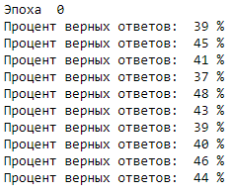
\includegraphics[width=0.4\linewidth]{./img/first-epoch}
  \caption{Начальное поколение нейронных сетей}
  \label{fig:mpr} 
\end{figure}

Поколение с номером 51 дает уже 73\% правильных ответов. Заметен существенный прирост в количестве верных ответов.

\begin{figure}[H]
  \centering
  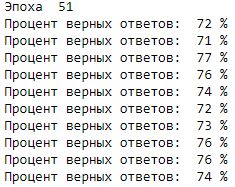
\includegraphics[width=0.4\linewidth]{./img/second-epoch}
  \caption{51 поколение нейронных сетей}
  \label{fig:mpr} 
\end{figure}

Последнее поколение будет отвечать на поставленную задачу правильно в 87\% случаев.

\begin{figure}[H]
  \centering
  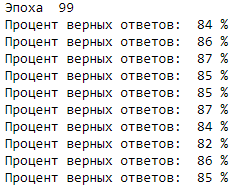
\includegraphics[width=0.4\linewidth]{./img/third-epoch}
  \caption{51 поколение нейронных сетей}
  \label{fig:mpr} 
\end{figure}

После прохождения 100 эпох получилась рабочая нейронная сеть, способная отвечать правильно на поставленную задачу в 87\% случаев.